\documentclass[12pt, a4paper]{article}
\usepackage[utf8]{inputenc}
\usepackage{graphicx}
\graphicspath{{img/}}

\usepackage[a4paper]{geometry}

\usepackage{caption}
\usepackage{tabularx}
\usepackage{booktabs}
\usepackage{subcaption}
%\usepackage{lscape}
\usepackage[table]{xcolor}
\usepackage{pbox}
\usepackage{array,booktabs}
\usepackage{multirow}
\usepackage{enumitem}
\usepackage{arydshln}
\usepackage{pdflscape}
\usepackage{colortbl}

\usepackage{forloop}% http://ctan.org/pkg/forloop
\newcounter{loopcntr}
\newcommand{\rpt}[2][1]{%
  \forloop{loopcntr}{0}{\value{loopcntr}<#1}{#2}%
}

%\usepackage[a4paper, left=3cm,right=3cm,top=2.5cm,bottom=2.5cm]{geometry}

\setlength{\parindent}{0pt} 
 
\begin{document}

\begin{titlepage}

\Large Pre project \\

\vspace{3cm}

\begin{center}
\Huge The analysis of C\# to F\# \vspace{10mm}\\
\large Jostein Andreassen, Michael Blomli and Mikkel Eltervåg \vspace{3mm}\\
Automation \vspace{5mm}\\
20. January 2015
\end{center}

\vspace{5cm}

\begin{figure}[!h]
  \centering
  \begin{minipage}[b]{0.3\textwidth}
    
\includegraphics[width=\textwidth]{fsharp128}
  \end{minipage}
  \hfill
  \begin{minipage}[b]{0.3\textwidth}
    
\includegraphics[width=\textwidth]{serit_logo}
  \end{minipage}
  \hfill
  \begin{minipage}[b]{0.3\textwidth}
    
\includegraphics[width=\textwidth]{LogoEngelsk}
  \end{minipage}
\end{figure}


\end{titlepage}

\tableofcontents

\newpage

\section{Background}
One of the biggest problems in modern application development is the rapidly growing complexity of all major software systems. This complexity makes it almost impossible to ensure the quality and accuracy of the code. It also becomes harder and harder to make changes to existing code without introducing new errors. All these difficulties multiply when you also want utilize modern computers with many CPU (central processing unit) cores for increased performance.\\

The imperative object-oriented programming paradigm has been dominant in software development for over 20 years. In the imperative paradigm the state variables will be handled explicitly, which can quickly give too much complexity. The functional programming paradigm has been known since the 1930’s, but has not been popular with professional developers because of the slightly lower (single core) performance and greater resource use. Today these obstacles are long gone, and functional programming is experiencing a new renaissance due to significantly better control over complexity and parallelism.\\

We've received an assignment from Serit to translate parts of an existing project from C\# code to F\# code. C\# is meant to be simple, modern, flexible and object oriented programming language. It  is developed and maintained by Microsoft and is inspired by previous popular object-oriented languages like C++ and Java. F\# is a hybrid language that supports both the familiar object-oriented method and functional programming. F\# is also developed by Microsoft, and like C\# also has access to Microsoft’s .NET framework. Serit wants us to find out the benefits of  switching from development in the programming language C\# development to F\#.\\

\newpage
\section{Problem for discussion}
C\# and F\# works in different ways, they both have benefits and downsides. The main question is if it is worth it for a company to change their main programming language. We have to look at what the company wants to achieve by making the change, and that boils down to making quality programs for a low price. \\

A modern IT company uses a lot of time developing, changing and fixing code. If we can use a programming language that takes less time to develop and at the same time works better without generating errors, that could be very cost saving.\\

The programming language F\# claims to be a solution to these problems by using less code, be more simple and have better error handling than other programming languages. Our task is to find out if those claims are true by answering these questions:

\begin{itemize}
\item What are the benefits of switching from C\# to F\#?
\item To what degree can we reduce the number of lines written in the program code?
\item How much time is saved in the debugging stage?
\item How much time is saved in the development of the code?
\end{itemize}

\newpage

\section{Formulations of objectives}
To work on an analysis (compare code) of the old code compared to the new code, where we will look at how compact the code is, how many errors there are, how self-explaining the code is and how easy it is to develop the code.

\newpage
\section{Project specification }

\subsection{Where Serit is now}

\begin{itemize}
	\item They have an ASP.NET Web application in C\# where the user interface is based on ASP Web Forms. All code is written in English, as well as all the text in the user interface.
	\item Language support is dissolved in a separate module sCore.Translation which is called from the application and performs translation according to data recorded in a translation table.
	\item Translation tables are located in a SQL database.

\end{itemize}

\begin{figure}[!h]
    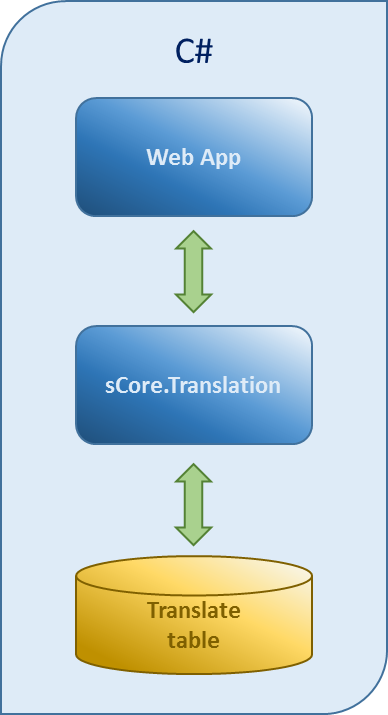
\includegraphics[scale=0.4]{image00}
    \centering
    \caption{How the communication of Serit's sCore.Translation application looks now.}
\end{figure}

\newpage
\subsection{What Serit wants}

\begin{itemize}
	\item They want to have the existing translation module sCore.Translation developed as a separate module in the functional language F\#. This should be able to be called from the present imperative program (C\#) and from functional programs (F\#).
	\item With the translation from C\# to F\# done, both languages and programming paradigms can be compared analytically. By this we can evaluate benefits (and possible disadvantages) with the functional paradigm in relation to an object-oriented imperative paradigm. The analysis will provide a better basis in the choice of programming language in future development projects.
\end{itemize}

\begin{figure}[!h]
    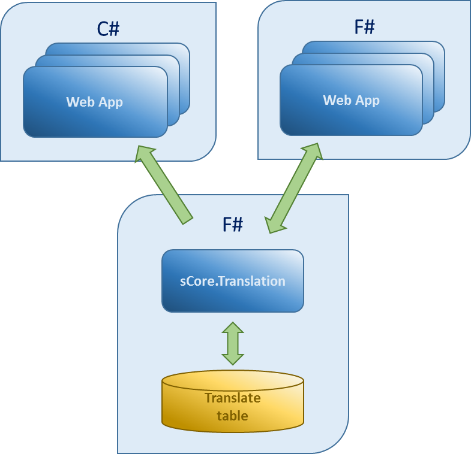
\includegraphics[scale=0.5]{image02}
    \centering
    \caption{How they want the sCore.Translation application to communicate.}
\end{figure}

\newpage
\subsection{Method of translation}
F\# for fun and profit describes three levels of “sophistication” for porting code from C\# to F\#. The basic level is simply a direct port. Since F\# supports imperative programming, we can translate directly. At the intermediate level, the code is refactored to be fully functional. The advanced level takes advantage of F\#’s data type system.\\

There are two paths to achieve this goal: Either by first porting to F\# and then refactoring to functional code, or by converting to functional code in C\# before porting that to F\#.

\begin{figure}[!h]
    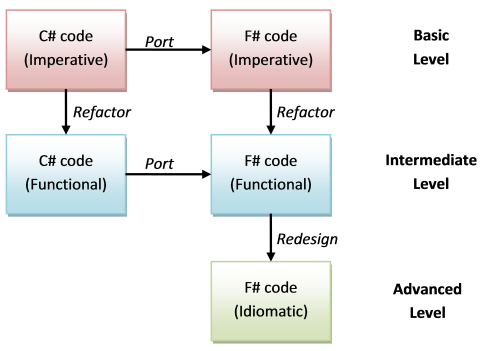
\includegraphics[scale=0.6]{image01}
    \centering
    \caption{Method's of translating from C\# to F\#.}
\end{figure}


\newpage
\section{Temporary table of contents for project report}
\begin{enumerate}
	\item First page
	\item Page 2
	\item Summary
	\item Foreword
	\item Table of contents
	\item Introduction 
	\begin{enumerate}
		\item Background
		\item Problem for discussion
		\item Formulation of objectives
	\end{enumerate}
	\item Main chapters
	\begin{enumerate}
		\item F\# programming language
		\item Imperative and functional programming
		\item Project specification
		\item Module A
		\begin{enumerate}
			\item Solution
			\item Analysis
		\end{enumerate}
		\item Module B, C…
		\begin{enumerate}
			\item Solution
			\item Analysis
		\end{enumerate}
		\item Complete analysis
		\begin{enumerate}
			\item Development time
			\item Readability and clarity
			\item Debugging and error handling
			\item Performance
		\end{enumerate}
	\end{enumerate}
	\item Conclusion
	\item Literature
	\item Attachments
	\begin{enumerate}
		\item Code
	\end{enumerate}
\end{enumerate}

\newpage
\section{Budget}
In this bachelor project we are going to use our own computers to write the code. Since the F\# is an open source software, and the C\# is free for community to use there is no need for a budget concerning software and hardware. The only thing that we can see for now that might be worth mentioning is the gasoline expense from driving between UiT and Serit (ca. 5 km one way if you check on google maps).\\

We found the rates for car driving on naf.no. They are as follows:\\

\begin{tabularx}{\textwidth}{|X|X|X|}
	\hline
	&Amount&Amount\\
	\hline
	Price per km&(1 - 10 000 km)&kr 4,10 / km\\
	\hline
	Additional passenger&1&kr 1,00\\
	\hline
\end{tabularx}\\

\vspace{5mm}

Actual cost:\\

\begin{tabularx}{\textwidth}{|p{50mm}|X|X|X|}
	\hline
	Expenses&Amount&Price&Sum\\
	\hline
	Driving from UiT to serit and back.&5 km * 2&kr 6,10 / km&kr 61,00\\
	\hline
	Status meetings at Serit each 7 days&20 Meetings&kr 61,00&kr 1220,00\\
	\hline
\end{tabularx}

\newpage
\section{Other resource needs}
Mostly we will do the programming for our self, where we can find much on the internet. Serit has offered us with assistance and try to help us with whatever we might need help with. We will mostly use Jonas as our mentor in F\#, because he is the go-to guy in that department. We will use Jens when it comes to the old existing software (program code) in C\#.

\subsection{Resource Contacts}
\begin{tabularx}{\textwidth}{|X|X|X|p{50mm}|}
	\hline
	Name&Company&Phone&Email\\
	\hline
	Sharma, Puneet&UiT&45063429&puneet.sharma@uit.no\\
	\hline
	Juselius, Jonas&Serit&&Jonas.Juselius@itpartner.no\\
	\hline
	Blomli, Jens&Serit&&Jens.Blomli@itpartner.no\\
	\hline
\end{tabularx}

\newpage
\section{Activity description}
All activities include the total number of hours for all 3 group members. We are expecting each member to contribute equally to all parts of the project.

\subsection{Activity list}

\begin{tabularx}{\textwidth}{|p{10mm}|X|X|p{10mm}|}
	\hline
	Act.nr&Act. name&Description&Dep.\\
	\hline
	C1&Initiation document&Send in initiation document&\\
	\hline
	B1&Learning fundamentals of F\#&Getting familiar with F\#&\\
	\hline
	A1&Status meeting&Meeting to check where we are at&\\
	\hline
	B2&Existing code&Get the code from Serit and check through it&\\
	\hline
	C2&Write pre-project&Start working on the pre-project document&C1\\
	\hline
	A2&Meeting with Serit&Meeting with Serit where they will talk about the project we are to make&\\
	\hline
	A3&Status meetings with Serit (ongoing)&Each monday there will be a status meeting&\\
	\hline
	B3&Set up Github accounts and learn Github&Get familiar with github and register accounts&\\
	\hline
	B4&Module: sTranslate&Start working on the project from Serit&B1, B2, B3\\
	\hline
	B4a&Set up test database&Set up a test database to test against&\\
	\hline
	B4b&Connect to test database with F\#&Make the database and F\# work together&B4a\\
	\hline
	B4c&Make F\# console app&Make a console application for the module&\\
	\hline
	B4d&Make the translate tool in F\#&Make the translate tool in F\#&B4b, B4c\\
	\hline
	B4e&Make F\# module compatible with C\# and .NET&Make the F\# translate tool available for C\#&B4d\\
	\hline
	B4f&Do a short analysis on the code&Make a short analysis of the sTransle module&B4e\\
	\hline
\end{tabularx}
	
\begin{tabularx}{\textwidth}{|p{10mm}|X|X|p{10mm}|}
	\hline
	A4&Meeting with mentor&Status meeting with mentor&\\
	\hline
	B5&Optional additional modules&If there is time, we will get more modules from Serit to work on&B4\\
	\hline
	C3&Deliver draft to UiT&Due date to deliver draft of project report&\\
	\hline
	C4&Write a complete analysis of F\# vs. C\#&Write the full analysis of F\# and C\#, pros and cons&B4, B5\\
	\hline
	A5&Posters for presentation&Make the posters for presentation&\\
	\hline
	A6&Course in presentation technique&Course in presentation technique will be offered for students&\\
	\hline
	A7&Presentation of project&The presentation of the projects in stands&\\
	\hline
	C5&Deliver project report&Due date for delivering project report&\\
	\hline
	C6&Deliver reflection notes&Due date for delivering reflection notes&\\
	\hline
	C7&Final presentation&Final presentation with individual examination&\\
	\hline
\end{tabularx}

\newpage

\subsection{Activities}

\small
\bgroup
\def\arraystretch{1.5}


% ---------------- C1 Initiation document ----------------
\begin{tabularx}{\textwidth}{|X|p{32mm}|p{20mm}|}
	\hline
	\textbf{Project:}&\textbf{Date:}&\textbf{Sign:}\\
	Basis for programming approach&20.01.2016&Jostein\\
	\hline
\end{tabularx}

\begin{tabularx}{\textwidth}{|p{40mm}|X|}
	\textbf{Akt. designation:}&\textbf{Name:}\\
	C1&Initiation document\\
	\hline
\end{tabularx}

\begin{tabularx}{\textwidth}{|X|}
	\textbf{Purpose:}\\
	To make a basis for starting on the pre-project, and to introduce the project to our mentor.\\
	\hline
	\textbf{Content / scope, procedure:}\\
	\begin{itemize}[noitemsep,topsep=0pt]
		\item Overview of background, problem, objectives and solution
		\item Plan work on the pre-project
		\item Due date 19.11.2015
 documents.
	\end{itemize}\\
 	\hline
	\textbf{Result:}\\
	 Approved initiation document\\
	\hline
\end{tabularx}

\begin{tabularx}{\textwidth}{|X|p{30mm}|}
	\textbf{Resource requirements:}&\textbf{Performed by:}\\
	72 hours&All\\
	\hline
\end{tabularx}

\newpage


% ---------------- B1 Learning some fundamentals ----------------
\begin{tabularx}{\textwidth}{|X|p{32mm}|p{20mm}|}
	\hline
	\textbf{Project:}&\textbf{Date:}&\textbf{Sign:}\\
	Basis for programming approach&20.01.2016&Jostein\\
	\hline
\end{tabularx}

\begin{tabularx}{\textwidth}{|p{40mm}|X|}
	\textbf{Akt. designation:}&\textbf{Name:}\\
	B1&Learning fundamentals of F\#\\
	\hline
\end{tabularx}

\begin{tabularx}{\textwidth}{|X|}
	\textbf{Purpose:}\\
	To familiarize with F\# and learn the basics of functional programming.\\
	\hline
	\textbf{Content / scope, procedure:}\\
	\begin{itemize}[noitemsep,topsep=0pt]
		\item Install F\# development tools
		\item Read/watch online tutorials
		\item Make some simple F\# programs
 programming.
	\end{itemize}\\
 	\hline
	\textbf{Result:}\\
	The team members understand the basic principles of functional programming, and can read and understand simple F\# code.\\
	\hline
\end{tabularx}

\begin{tabularx}{\textwidth}{|X|p{30mm}|}
	\textbf{Resource requirements:}&\textbf{Performed by:}\\
	30 hours per week over 4 weeks&All\\
	\hline
\end{tabularx}

\newpage

% ---------------- A1 Status meeting ----------------
\begin{tabularx}{\textwidth}{|X|p{32mm}|p{20mm}|}
	\hline
	\textbf{Project:}&\textbf{Date:}&\textbf{Sign:}\\
	Basis for programming approach&20.01.2016&Jostein\\
	\hline
\end{tabularx}

\begin{tabularx}{\textwidth}{|p{40mm}|X|}
	\textbf{Akt. designation:}&\textbf{Name:}\\
	A1&Status meeting\\
	\hline
\end{tabularx}

\begin{tabularx}{\textwidth}{|X|}
	\textbf{Purpose:}\\
	Status meeting after the holidays to plan work on the pre-project.\\
	\hline
	\textbf{Content / scope, procedure:}\\
	\begin{itemize}[noitemsep,topsep=0pt]
		\item Meeting date 06.01.2016
		\item Follow-up on activity B1
		\item Planning for pre-project 
	\end{itemize}\\
 	\hline
	\textbf{Result:}\\
	Roadmap for pre-project work.\\
	\hline
\end{tabularx}

\begin{tabularx}{\textwidth}{|X|p{30mm}|}
	\textbf{Resource requirements:}&\textbf{Performed by:}\\
	6 hours&All\\
	\hline
\end{tabularx}

\newpage

% ---------------- B2 Existing code ----------------
\begin{tabularx}{\textwidth}{|X|p{32mm}|p{20mm}|}
	\hline
	\textbf{Project:}&\textbf{Date:}&\textbf{Sign:}\\
	Basis for programming approach&20.01.2016&Jostein\\
	\hline
\end{tabularx}

\begin{tabularx}{\textwidth}{|p{40mm}|X|}
	\textbf{Akt. designation:}&\textbf{Name:}\\
	B2&Existing code\\
	\hline
\end{tabularx}

\begin{tabularx}{\textwidth}{|X|}
	\textbf{Purpose:}\\
	To develop an understanding of the existing C\# code.\\
	\hline
	\textbf{Content / scope, procedure:}\\
	\begin{itemize}
		\item Read the code which Serit has released on Github
		\item Discuss it with the rest of the team members
\end{itemize}\\
 	\hline
	\textbf{Result:}\\
	The team members understand the purpose and functionality of the code\\
	\hline
\end{tabularx}

\begin{tabularx}{\textwidth}{|X|p{30mm}|}
	\textbf{Resource requirements:}&\textbf{Performed by:}\\
	30 hours&All\\
	\hline
\end{tabularx}

\newpage

% ---------------- C2 Pre-project ----------------
\begin{tabularx}{\textwidth}{|X|p{32mm}|p{20mm}|}
	\hline
	\textbf{Project:}&\textbf{Date:}&\textbf{Sign:}\\
	Basis for programming approach&20.01.2016&Mikkel\\
	\hline
\end{tabularx}

\begin{tabularx}{\textwidth}{|p{40mm}|X|}
	\textbf{Akt. designation:}&\textbf{Name:}\\
	C2&Pre-project\\
	\hline
\end{tabularx}

\begin{tabularx}{\textwidth}{|X|}
	\textbf{Purpose:}\\
	To get a good plan before starting on the project.\\
	\hline
	\textbf{Content / scope, procedure:}\\
	\begin{itemize}[noitemsep,topsep=0pt]
		\item Get information from Serit about how to conduct the project
		\item Plan and discuss what our plan for the project is
		\item Formulate the problem and objectives clearly
		\item Write a detailed activity description
		\item Gantt-diagram
		\item Due date 20.01.2016


	\end{itemize}\\
 	\hline
	\textbf{Result:}\\
	A written plan and a good base before starting on the project.\\
	\hline
\end{tabularx}

\begin{tabularx}{\textwidth}{|X|p{30mm}|}
	\textbf{Resource requirements:}&\textbf{Performed by:}\\
	45 hours&All\\
	\hline
\end{tabularx}

\newpage

% ---------------- A2 Meeting with Serit ----------------
\begin{tabularx}{\textwidth}{|X|p{32mm}|p{20mm}|}
	\hline
	\textbf{Project:}&\textbf{Date:}&\textbf{Sign:}\\
	Basis for programming approach&20.01.2016&Mikkel\\
	\hline
\end{tabularx}

\begin{tabularx}{\textwidth}{|p{40mm}|X|}
	\textbf{Akt. designation:}&\textbf{Name:}\\
	A2&Meeting with Serit\\
	\hline
\end{tabularx}

\begin{tabularx}{\textwidth}{|X|}
	\textbf{Purpose:}\\
	Get a presentation of the code we are going to translate.\\
	\hline
	\textbf{Content / scope, procedure:}\\
	\begin{itemize}[noitemsep,topsep=0pt]
		\item Meeting date 18.01.2016
		\item Get information about the code we are going 			\item Learn how they want the structure and the syntax to be
		\item Learn more F\#
		\item Plan future meetings

	\end{itemize}\\
 	\hline
	\textbf{Result:}\\
	Get enough information about the project that we can start working on the translation of the code.\\
	\hline
\end{tabularx}

\begin{tabularx}{\textwidth}{|X|p{30mm}|}
	\textbf{Resource requirements:}&\textbf{Performed by:}\\
	 6 hours&All\\
	\hline
\end{tabularx}

\newpage

% ---------------- A3 Status meetings with Serit (ongoing) ----------------
\begin{tabularx}{\textwidth}{|X|p{32mm}|p{20mm}|}
	\hline
	\textbf{Project:}&\textbf{Date:}&\textbf{Sign:}\\
	Basis for programming approach&20.01.2016&Michael\\
	\hline
\end{tabularx}

\begin{tabularx}{\textwidth}{|p{40mm}|X|}
	\textbf{Akt. designation:}&\textbf{Name:}\\
	A3&Status meetings with Serit (ongoing)\\
	\hline
\end{tabularx}

\begin{tabularx}{\textwidth}{|X|}
	\textbf{Purpose:}\\
	A meeting to check where we are at and if we are as scheduled.\\
	\hline
	\textbf{Content / scope, procedure:}\\
	\begin{itemize}[noitemsep,topsep=0pt]
		\item Status meeting each monday with serit.
	\end{itemize}\\
 	\hline
	\textbf{Result:}\\
	Check our current status.\\
	\hline
\end{tabularx}

\begin{tabularx}{\textwidth}{|X|p{30mm}|}
	\textbf{Resource requirements:}&\textbf{Performed by:}\\
	6 hours per week for 9 weeks&All\\
	\hline
\end{tabularx}

\newpage

% ---------------- B3 Set up Github accounts and learn Github ----------------
\begin{tabularx}{\textwidth}{|X|p{32mm}|p{20mm}|}
	\hline
	\textbf{Project:}&\textbf{Date:}&\textbf{Sign:}\\
	Basis for programming approach&20.01.2016&Mikkel\\
	\hline
\end{tabularx}

\begin{tabularx}{\textwidth}{|p{40mm}|X|}
	\textbf{Akt. designation:}&\textbf{Name:}\\
	B3&Set up Github accounts and learn Github\\
	\hline
\end{tabularx}

\begin{tabularx}{\textwidth}{|X|}
	\textbf{Purpose:}\\
	To get a good platform for sharing code files in a organized way.\\
	\hline
	\textbf{Content / scope, procedure:}\\
	\begin{itemize}[noitemsep,topsep=0pt]
		\item Set up a group account on Github
		\item Learn the all the basic of Github
 		\item Find the best way to use Github with Visual Studio
		\item Connect and get files from Serit’s Github

	\end{itemize}\\
 	\hline
	\textbf{Result:}\\
	Good knowledge of Github and a good and easy way to handle the files in the project.\\
	\hline
\end{tabularx}

\begin{tabularx}{\textwidth}{|X|p{30mm}|}
	\textbf{Resource requirements:}&\textbf{Performed by:}\\
	15 hours&All\\
	\hline
\end{tabularx}

\newpage

% ---------------- B4 Module: sTranslate  ----------------
\begin{tabularx}{\textwidth}{|X|p{32mm}|p{20mm}|}
	\hline
	\textbf{Project:}&\textbf{Date:}&\textbf{Sign:}\\
	Basis for programming approach&20.01.16&Jostein\\
	\hline
\end{tabularx}

\begin{tabularx}{\textwidth}{|p{40mm}|X|}
	\textbf{Akt. designation:}&\textbf{Name:}\\
	B4&Module: sTranslate \\
	\hline
\end{tabularx}

\begin{tabularx}{\textwidth}{|X|}
	\textbf{Purpose:}\\
	To make an F\# version of the sTranslate module provided by Serit.\\
	\hline
	\textbf{Content / scope, procedure:}\\
	Sub-activities:\\
	\begin{itemize}[noitemsep,topsep=0pt]
		\item B4a - Set up test database
		\item B4b - Connect to test database with F\#
		\item B4c - Make F\# console app
		\item B4d - Make the translate tool in F\#
		\item B4e - Make F\# module compatible with C\# and .NET
		\item B4f - Do a short analysis on the code.


	\end{itemize}\\
 	\hline
	\textbf{Result:}\\
	A working F\# implementation of the C\# module provided by Serit, as well as a short analysis and summary.\\
	\hline
\end{tabularx}

\begin{tabularx}{\textwidth}{|X|p{30mm}|}
	\textbf{Resource requirements:}&\textbf{Performed by:}\\
	 Refer to sub-activities&All\\
	\hline
\end{tabularx}

\newpage

% ---------------- B4a To set up a database used for testing the sTranslate module  ----------------
\begin{tabularx}{\textwidth}{|X|p{32mm}|p{20mm}|}
	\hline
	\textbf{Project:}&\textbf{Date:}&\textbf{Sign:}\\
	Basis for programming approach&20.01.2016&Jostein\\
	\hline
\end{tabularx}

\begin{tabularx}{\textwidth}{|p{40mm}|X|}
	\textbf{Akt. designation:}&\textbf{Name:}\\
	B4a&To set up a database \\
	\hline
\end{tabularx}

\begin{tabularx}{\textwidth}{|X|}
	\textbf{Purpose:}\\
	To set up a database used for testing the sTranslate module.\\
	\hline
	\textbf{Content / scope, procedure:}\\
	\begin{itemize}
		\item We will be provided with SQL files for creating a translation database that will be used to test the sTranslate module. We will set up and run this database locally for use in testing.
	\end{itemize} \\
 	\hline
	\textbf{Result:}\\
	The database is running and working as intended. \\
	\hline
\end{tabularx}

\begin{tabularx}{\textwidth}{|X|p{30mm}|}
	\textbf{Resource requirements:}&\textbf{Performed by:}\\
	15 hours&All\\
	\hline
\end{tabularx}

\newpage

% ---------------- B4b Connect to test database with F\#  ----------------
\begin{tabularx}{\textwidth}{|X|p{32mm}|p{20mm}|}
	\hline
	\textbf{Project:}&\textbf{Date:}&\textbf{Sign:}\\
	Basis for programming approach&20.01.2016&Jostein\\
	\hline
\end{tabularx}

\begin{tabularx}{\textwidth}{|p{40mm}|X|}
	\textbf{Akt. designation:}&\textbf{Name:}\\
	B4b&Connect to test database with F\# \\
	\hline
\end{tabularx}

\begin{tabularx}{\textwidth}{|X|}
	\textbf{Purpose:}\\
	Create a very simple F\# program to run SQL queries on the database.\\
	\hline
	\textbf{Content / scope, procedure:}\\
	\begin{itemize}
		\item We will access the test database using F\# Type Providers. We will write a simple program and get some data out of the database.
	\end{itemize}\\
 	\hline
	\textbf{Result:}\\
	We are able to retrieve information from the database using F\#. \\
	\hline
\end{tabularx}

\begin{tabularx}{\textwidth}{|X|p{30mm}|}
	\textbf{Resource requirements:}&\textbf{Performed by:}\\
	30 hours&All\\
	\hline
\end{tabularx}

\newpage

% ---------------- B4c Make the F\# console app  ----------------
\begin{tabularx}{\textwidth}{|X|p{32mm}|p{20mm}|}
	\hline
	\textbf{Project:}&\textbf{Date:}&\textbf{Sign:}\\
	Basis for programming approach&20.01.2016&Jostein\\
	\hline
\end{tabularx}

\begin{tabularx}{\textwidth}{|p{40mm}|X|}
	\textbf{Akt. designation:}&\textbf{Name:}\\
	B4c&Make the F\# console app \\
	\hline
\end{tabularx}

\begin{tabularx}{\textwidth}{|X|}
	\textbf{Purpose:}\\
	To create a test app with input and output functionality.\\
	\hline
	\textbf{Content / scope, procedure:}\\
	\begin{itemize}
		\item We will make a simple console application to test the program. It should take input in the correct format and give the correct output.
	\end{itemize}\\
 	\hline
	\textbf{Result:}\\
	The console app is working. \\
	\hline
\end{tabularx}

\begin{tabularx}{\textwidth}{|X|p{30mm}|}
	\textbf{Resource requirements:}&\textbf{Performed by:}\\
	45 hours per week for 2 weeks&All\\
	\hline
\end{tabularx}

\newpage

% ---------------- B4d Make the translate tool in F\#  ----------------
\begin{tabularx}{\textwidth}{|X|p{32mm}|p{20mm}|}
	\hline
	\textbf{Project:}&\textbf{Date:}&\textbf{Sign:}\\
	Basis for programming approach&20.01.2016&Jostein\\
	\hline
\end{tabularx}

\begin{tabularx}{\textwidth}{|p{40mm}|X|}
	\textbf{Akt. designation:}&\textbf{Name:}\\
	B4d&Make the translate tool in F\# \\
	\hline
\end{tabularx}

\begin{tabularx}{\textwidth}{|X|}
	\textbf{Purpose:}\\
	To implement the translate tool in F\#.\\
	\hline
	\textbf{Content / scope, procedure:}\\
	\begin{itemize}
		\item The translate tool is the program that will actually do the SQL query to the database. It will be called from the console app and return the correct translation.
	\end{itemize}\\
 	\hline
	\textbf{Result:}\\
	The translate tool can be called from the test app, and return the correct translation. \\
	\hline
\end{tabularx}

\begin{tabularx}{\textwidth}{|X|p{30mm}|}
	\textbf{Resource requirements:}&\textbf{Performed by:}\\
	45 hours per week for 3 weeks&All\\
	\hline
\end{tabularx}

\newpage

% ---------------- B4e To make our F\# module compatible with the rest of Serit’s code, which is C\#   ----------------
\begin{tabularx}{\textwidth}{|X|p{32mm}|p{20mm}|}
	\hline
	\textbf{Project:}&\textbf{Date:}&\textbf{Sign:}\\
	Basis for programming approach&20.01.2016&Jostein\\
	\hline
\end{tabularx}

\begin{tabularx}{\textwidth}{|p{40mm}|X|}
	\textbf{Akt. designation:}&\textbf{Name:}\\
	B4e&Make F\# module compatible with C\# and .NET \\
	\hline
\end{tabularx}

\begin{tabularx}{\textwidth}{|X|}
	\textbf{Purpose:}\\
	To implement the translate tool in F\#.\\
	\hline
	\textbf{Content / scope, procedure:}\\
	\begin{itemize}
		\item Serit’s entire project is written in C\#. They should be able to call on our module without any problems.
		\item We will need to make sure our module is compatible. 
	\end{itemize}\\
 	\hline
	\textbf{Result:}\\
	The module is successfully used with the existing code. \\
	\hline
\end{tabularx}

\begin{tabularx}{\textwidth}{|X|p{30mm}|}
	\textbf{Resource requirements:}&\textbf{Performed by:}\\
	10 hours per week for 3 weeks
&All\\
	\hline
\end{tabularx}

\newpage

% ---------------- B4f Do a short analysis on the code   ----------------
\begin{tabularx}{\textwidth}{|X|p{32mm}|p{20mm}|}
	\hline
	\textbf{Project:}&\textbf{Date:}&\textbf{Sign:}\\
	Basis for programming approach&20.01.2016&Jostein\\
	\hline
\end{tabularx}

\begin{tabularx}{\textwidth}{|p{40mm}|X|}
	\textbf{Akt. designation:}&\textbf{Name:}\\
	B4f&Do a short analysis on the code  \\
	\hline
\end{tabularx}

\begin{tabularx}{\textwidth}{|X|}
	\textbf{Purpose:}\\
	To make some groundwork for the final analysis.\\
	\hline
	\textbf{Content / scope, procedure:}\\
	Note any problems/difficulties we had when implementing these features in F\#
Compare the program code for C\# and F\#: \\
	\begin{itemize}
		\item Length
		\item Readability
		\item Conciseness
	\end{itemize}
	See if there are any differences in performance (it’s a small program, but if it must be called many times it should be fast).\\
 	\hline
	\textbf{Result:}\\
	A short analysis and comparison. \\
	\hline
\end{tabularx}

\begin{tabularx}{\textwidth}{|X|p{30mm}|}
	\textbf{Resource requirements:}&\textbf{Performed by:}\\
	45 hours&All\\
	\hline
\end{tabularx}

\newpage

% ---------------- A4 Meeting with mentor   ----------------
\begin{tabularx}{\textwidth}{|X|p{32mm}|p{20mm}|}
	\hline
	\textbf{Project:}&\textbf{Date:}&\textbf{Sign:}\\
	Basis for programming approach&20.01.2016&Jostein\\
	\hline
\end{tabularx}

\begin{tabularx}{\textwidth}{|p{40mm}|X|}
	\textbf{Akt. designation:}&\textbf{Name:}\\
	A4&Meeting with mentor  \\
	\hline
\end{tabularx}

\begin{tabularx}{\textwidth}{|X|}
	\textbf{Purpose:}\\
	For the mentor to see that work on the project is coming along well\\
	\hline
	\textbf{Content / scope, procedure:}\\
	\begin{itemize}
		\item Have a status meeting with our mentor 
		\item The mentor will call a meeting in February

	\end{itemize}\\
 	\hline
	\textbf{Result:}\\
	Progress overview\\
	\hline
\end{tabularx}

\begin{tabularx}{\textwidth}{|X|p{30mm}|}
	\textbf{Resource requirements:}&\textbf{Performed by:}\\
	6 hours&All\\
	\hline
\end{tabularx}

\newpage

% ---------------- B5 Optional additional modules   ----------------
\begin{tabularx}{\textwidth}{|X|p{32mm}|p{20mm}|}
	\hline
	\textbf{Project:}&\textbf{Date:}&\textbf{Sign:}\\
	Basis for programming approach&20.01.2016&Jostein\\
	\hline
\end{tabularx}

\begin{tabularx}{\textwidth}{|p{40mm}|X|}
	\textbf{Akt. designation:}&\textbf{Name:}\\
	B5&Optional additional modules  \\
	\hline
\end{tabularx}

\begin{tabularx}{\textwidth}{|X|}
	\textbf{Purpose:}\\
	Port additional modules to F\# code.\\
	\hline
	\textbf{Content / scope, procedure:}\\
	\begin{itemize}
		\item Depending on available time, we will translate more modules from the same project into F\#. We will use the same procedure as in activity A-7.
	\end{itemize}\\
 	\hline
	\textbf{Result:}\\
	Additional F\# modules and code to base the final analysis on. \\
	\hline
\end{tabularx}

\begin{tabularx}{\textwidth}{|X|p{30mm}|}
	\textbf{Resource requirements:}&\textbf{Performed by:}\\
	90 hours per week over 3 weeks&All\\
	\hline
\end{tabularx}

\newpage

% ---------------- C3 Deliver draft to UiT   ----------------
\begin{tabularx}{\textwidth}{|X|p{32mm}|p{20mm}|}
	\hline
	\textbf{Project:}&\textbf{Date:}&\textbf{Sign:}\\
	Basis for programming approach&11.04.16&Michael\\
	\hline
\end{tabularx}

\begin{tabularx}{\textwidth}{|p{40mm}|X|}
	\textbf{Akt. designation:}&\textbf{Name:}\\
	C3&Deliver draft to UiT  \\
	\hline
\end{tabularx}

\begin{tabularx}{\textwidth}{|X|}
	\textbf{Purpose:}\\
	 We will make a draft of the project report so we can get feedback and see if we’ve achieved our goals.\\
	\hline
	\textbf{Content / scope, procedure:}\\
	\begin{itemize}
		\item We will use the completed work to write the draft, and skip items where we don’t have anything to write.
		\item Explain problem and formulation of objectives.
		\item Describe the programming languages used and the different programming paradigms.
		\item Explain how we completed the task from Serit.
		\item Note any issues we had during work on the project, and how we solved these.
		\item Any deviations from the plan in the pre-project.
		\item Discuss our result and compare it to our objectives.
		\item How could we have avoided issues and what could have been done differently.
		\item Was the project successful or not (did we achieve our objective, and did we learn anything?)
		\item Due date 11.04.2016

	\end{itemize}\\
 	\hline
	\textbf{Result:}\\
	Completed and documented project \\
	\hline
\end{tabularx}

\begin{tabularx}{\textwidth}{|X|p{30mm}|}
	\textbf{Resource requirements:}&\textbf{Performed by:}\\
	30 hours per week for 3 weeks&All\\
	\hline
\end{tabularx}

\newpage

% ---------------- C4 Write a complete analysis of F# vs. C#   ----------------
\begin{tabularx}{\textwidth}{|X|p{32mm}|p{20mm}|}
	\hline
	\textbf{Project:}&\textbf{Date:}&\textbf{Sign:}\\
	Basis for programming approach&20.01.2016&Mikkel\\
	\hline
\end{tabularx}

\begin{tabularx}{\textwidth}{|p{40mm}|X|}
	\textbf{Akt. designation:}&\textbf{Name:}\\
	C4&Write a complete analysis of F\# vs. C\#  \\
	\hline
\end{tabularx}

\begin{tabularx}{\textwidth}{|X|}
	\textbf{Purpose:}\\
	Finding out the benefits of using F\# instead of C\#.\\
	\hline
	\textbf{Content / scope, procedure:}\\
	\begin{itemize}
		\item Look at the amount of code used in the coding languages.
		\item Estimate the amount of bugs that can happen in the coding languages.
		\item Estimate the time used development using C\# and F\#.
		\item Discuss if it’s worth training developers to use this new language..
		\item Make tables and visual data ready for the final project report
		\item Complete by 14.04.16
	\end{itemize}\\
 	\hline
	\textbf{Result:}\\
	Data that are ready to be used in the final report. \\
	\hline
\end{tabularx}

\begin{tabularx}{\textwidth}{|X|p{30mm}|}
	\textbf{Resource requirements:}&\textbf{Performed by:}\\
	80 hours per week for 4 weeks&All\\
	\hline
\end{tabularx}

\newpage

% ---------------- A5 Posters for presentation   ----------------
\begin{tabularx}{\textwidth}{|X|p{32mm}|p{20mm}|}
	\hline
	\textbf{Project:}&\textbf{Date:}&\textbf{Sign:}\\
	Basis for programming approach&20.01.2016&Michael\\
	\hline
\end{tabularx}

\begin{tabularx}{\textwidth}{|p{40mm}|X|}
	\textbf{Akt. designation:}&\textbf{Name:}\\
	A5&Posters for presentation  \\
	\hline
\end{tabularx}

\begin{tabularx}{\textwidth}{|X|}
	\textbf{Purpose:}\\
	The posters for the presentation must be printed.\\
	\hline
	\textbf{Content / scope, procedure:}\\
	\begin{itemize}
		\item Discuss and design the concept for our stand
		\item Prepare the presentation
		\item Show our work in an understandable way
		\item Easy graphical presentations to make the results very clear
		\item Hand in the produced poster for printing no later than 15.04.2016

	\end{itemize}\\
 	\hline
	\textbf{Result:}\\
	Posters to use at the presentation \\
	\hline
\end{tabularx}

\begin{tabularx}{\textwidth}{|X|p{30mm}|}
	\textbf{Resource requirements:}&\textbf{Performed by:}\\
	30 hours&All\\
	\hline
\end{tabularx}

\newpage

% ---------------- A6 Course in presentation technique   ----------------
\begin{tabularx}{\textwidth}{|X|p{32mm}|p{20mm}|}
	\hline
	\textbf{Project:}&\textbf{Date:}&\textbf{Sign:}\\
	Basis for programming approach&20.01.2016&Jostein\\
	\hline
\end{tabularx}

\begin{tabularx}{\textwidth}{|p{40mm}|X|}
	\textbf{Akt. designation:}&\textbf{Name:}\\
	A6&Course in presentation technique  \\
	\hline
\end{tabularx}

\begin{tabularx}{\textwidth}{|X|}
	\textbf{Purpose:}\\
	To improve our presentation skills before the oral presentation in June.\\
	\hline
	\textbf{Content / scope, procedure:}\\
	\begin{itemize}
		\item Follow course in presentation technique
		\item Learn and get better presenting a project
		\item Discuss and practice presenting
		\item The course will be from 19. - 22. April
	\end{itemize}\\
 	\hline
	\textbf{Result:}\\
	Increased presentation skills \\
	\hline
\end{tabularx}

\begin{tabularx}{\textwidth}{|X|p{30mm}|}
	\textbf{Resource requirements:}&\textbf{Performed by:}\\
	24 hours&All\\
	\hline
\end{tabularx}

\newpage

% ---------------- A7 Presentation of project   ----------------
\begin{tabularx}{\textwidth}{|X|p{32mm}|p{20mm}|}
	\hline
	\textbf{Project:}&\textbf{Date:}&\textbf{Sign:}\\
	Basis for programming approach&20.01.2016&Michael\\
	\hline
\end{tabularx}

\begin{tabularx}{\textwidth}{|p{40mm}|X|}
	\textbf{Akt. designation:}&\textbf{Name:}\\
	A7&Presentation of project  \\
	\hline
\end{tabularx}

\begin{tabularx}{\textwidth}{|X|}
	\textbf{Purpose:}\\
	To present the project for others\\
	\hline
	\textbf{Content / scope, procedure:}\\
	\begin{itemize}
		\item Practice the presentation
		\item Presentation length should be around 10 minutes
		\item Explain who we are and our problem formulation
		\item Explain the background of the project
		\item Explain the basics of object-oriented programming and functional programming
		\item Take into consideration that our audience probably knows much less about programming than us.
		\item Avoid in-depth technical details
		\item Answer questions after the presentation, and at the stand
		\item Presentation date: 28.04.2016

	\end{itemize}\\
 	\hline
	\textbf{Result:}\\
	Completed presentation \\
	\hline
\end{tabularx}

\begin{tabularx}{\textwidth}{|X|p{30mm}|}
	\textbf{Resource requirements:}&\textbf{Performed by:}\\
	30 hours per week over 2 weeks&All\\
	\hline
\end{tabularx}

\newpage

% ---------------- C5 Deliver project report   ----------------
\begin{tabularx}{\textwidth}{|X|p{32mm}|p{20mm}|}
	\hline
	\textbf{Project:}&\textbf{Date:}&\textbf{Sign:}\\
	Basis for programming approach&20.01.2016&Michael\\
	\hline
\end{tabularx}

\begin{tabularx}{\textwidth}{|p{40mm}|X|}
	\textbf{Akt. designation:}&\textbf{Name:}\\
	C5&Deliver project report  \\
	\hline
\end{tabularx}

\begin{tabularx}{\textwidth}{|X|}
	\textbf{Purpose:}\\
	 The written project report serves as the documentation for the project\\
	\hline
	\textbf{Content / scope, procedure:}\\
	\begin{itemize}
		\item Read through feedback from the draft 
		\item Discuss how we can improve the report
		\item Add missing stuff
		\item Eventual changes
		\item Due-date to deliver the final project report (Electronic): 12.05.2016

	\end{itemize}\\
 	\hline
	\textbf{Result:}\\
	Delivered project report \\
	Completed project\\
	\hline
\end{tabularx}

\begin{tabularx}{\textwidth}{|X|p{30mm}|}
	\textbf{Resource requirements:}&\textbf{Performed by:}\\
	70 hours per week for 3 weeks&All\\
	\hline
\end{tabularx}

\newpage

% ---------------- C6 Deliver reflection notes   ----------------
\begin{tabularx}{\textwidth}{|X|p{32mm}|p{20mm}|}
	\hline
	\textbf{Project:}&\textbf{Date:}&\textbf{Sign:}\\
	Basis for programming approach&20.01.2016&Michael\\
	\hline
\end{tabularx}

\begin{tabularx}{\textwidth}{|p{40mm}|X|}
	\textbf{Akt. designation:}&\textbf{Name:}\\
	C6&Deliver reflection notes  \\
	\hline
\end{tabularx}

\begin{tabularx}{\textwidth}{|X|}
	\textbf{Purpose:}\\
	 To summarize and reflect on what we have done.\\
	\hline
	\textbf{Content / scope, procedure:}\\
	\begin{itemize}
		\item Describe our experience with the project work
		\item Discuss if we achieved our goals/objectives
		\item Discuss if we managed to stay on the schedule we planned in the pre-project
		\item Due-date to deliver reflection notes: 18.05.2016

	\end{itemize}\\
 	\hline
	\textbf{Result:}\\
	Overview of project completion and results \\
	\hline
\end{tabularx}

\begin{tabularx}{\textwidth}{|X|p{30mm}|}
	\textbf{Resource requirements:}&\textbf{Performed by:}\\
	30 hours&All\\
	\hline
\end{tabularx}

\newpage

% ---------------- C7 Final presentation with individual examination   ----------------
\begin{tabularx}{\textwidth}{|X|p{32mm}|p{20mm}|}
	\hline
	\textbf{Project:}&\textbf{Date:}&\textbf{Sign:}\\
	Basis for programming approach&20.01.2016&Jostein\\
	\hline
\end{tabularx}

\begin{tabularx}{\textwidth}{|p{40mm}|X|}
	\textbf{Akt. designation:}&\textbf{Name:}\\
	C7&Final presentation with individual examination  \\
	\hline
\end{tabularx}

\begin{tabularx}{\textwidth}{|X|}
	\textbf{Purpose:}\\
	 To present our project\\
	\hline
	\textbf{Content / scope, procedure:}\\
	\begin{itemize}
		\item Condense the project report to a short oral presentation
		\item Our audience will be professionals with relevant education
		\item Presentation length including questions will be 45 min.
		\item Practice the presentation as a group
		\item Individual examinations 9. and 10. of June
	\end{itemize}\\
 	\hline
	\textbf{Result:}\\
	Completed presentation for individual examination \\
	\hline
\end{tabularx}

\begin{tabularx}{\textwidth}{|X|p{30mm}|}
	\textbf{Resource requirements:}&\textbf{Performed by:}\\
	25 hours per week for 4 weeks&All\\
	\hline
\end{tabularx}

\egroup



\newgeometry{left=3cm,right=3cm,top=2.5cm,bottom=2.5cm}
\begin{landscape}
\subsection{Gantt-Diagram}
\footnotesize
\begin{tabularx}{\textwidth}{l|c:c:c:c:c:c:c:c:c:c:c:c:c:c:c:c:c:c:c:c:c:c:c:c:c:c:}
	&\multicolumn{10}{l}{Week number}\\
	Activity&51&52&53&1&2&3&4&5&6&7&8&9&10&11&12&13&14&15&16&17&18&19&20&21&22&23\\
  	
  	\rpt[26]{&}\\
  	  	
  	
  	\hdashline
  	
  	C1 Initiation document
  		\rpt[1]{&\cellcolor{red!25}}
  		\rpt[25]{&}\\
  	
  	\hdashline
  	
  	B1 Learning some fundamentals
  		\rpt[5]{&\cellcolor{blue!50}}
  		\rpt[21]{&}\\
  		
  	\hdashline
  	
  	A1 Status meeting
  		\rpt[4]{&}
  		\rpt[1]{&\cellcolor{green!25}}
  		\rpt[21]{&}\\
  		
  	\hdashline
  	
  	B2 Existing code
  		\rpt[5]{&}
  		\rpt[3]{&\cellcolor{blue!50}}
  		\rpt[18]{&}\\
  		
  	\hdashline
  	
  	C2 Pre-project
  		\rpt[4]{&}
  		\rpt[2]{&\cellcolor{red!25}}
  		\rpt[20]{&}\\
  		
  	\hdashline
  	
  	A2 Meeting with Serit
  		\rpt[6]{&}
  		\rpt[1]{&\cellcolor{green!25}}
  		\rpt[19]{&}\\
  		
  		
  	\hdashline
  	
  	A3 Status meetings with Serit
  		\rpt[7]{&}
  		\rpt[9]{&\cellcolor{green!25}}
  		\rpt[10]{&}\\
  		
  	\hdashline
  	
  	B3 Learn Github and set up
  		\rpt[7]{&}
  		\rpt[3]{&\cellcolor{blue!50}}
  		\rpt[16]{&}\\
  		
  	\hdashline
  	
  	B4 Module: sTranslate
  		\rpt[7]{&}
  		\rpt[5]{&\cellcolor{blue!50}}
  		\rpt[14]{&}\\
  		
  	\hdashline
  	
  	B4a Set up and test sTranslate
  		\rpt[7]{&}
  		\rpt[1]{&\cellcolor{blue!50}}
  		\rpt[18]{&}\\
  		
  	\hdashline
  	
  	B4b Connect database
  		\rpt[7]{&}
  		\rpt[1]{&\cellcolor{blue!50}}
  		\rpt[18]{&}\\
  		
  	\hdashline
  	
  	B4c F\# console app
  		\rpt[7]{&}
  		\rpt[2]{&\cellcolor{blue!50}}
  		\rpt[17]{&}\\
  		
  	\hdashline
  	
  	B4d F\# translate tool
  		\rpt[8]{&}
  		\rpt[3]{&\cellcolor{blue!50}}
  		\rpt[15]{&}\\
  		
  	\hdashline
  	
  	B4e C\# compatibility
  		\rpt[9]{&}
  		\rpt[2]{&\cellcolor{blue!50}}
  		\rpt[15]{&}\\
  		
  	\hdashline
  	
  	B4f Analysis of sTranslate
  		\rpt[11]{&}
  		\rpt[1]{&\cellcolor{blue!50}}
  		\rpt[14]{&}\\
  		
  	\hdashline
  	
  	A4 Meeting with mentor
  		\rpt[8]{&}
  		\rpt[4]{&\cellcolor{green!25}}
  		\rpt[14]{&}\\
  		
  	\hdashline
  	
  	B5 Optional modules
  		\rpt[12]{&}
  		\rpt[3]{&\cellcolor{blue!50}}
  		\rpt[9]{&}\\
  		
  	\hdashline
  	
  	C3 Deliver draft
  		\rpt[14]{&}
  		\rpt[3]{&\cellcolor{red!25}}
  		\rpt[9]{&}\\
  		
  	\hdashline
  	
  	C4 Complete analysis
  		\rpt[15]{&}
  		\rpt[4]{&\cellcolor{red!25}}
  		\rpt[7]{&}\\
  		
  	\hdashline
  	
  	A5 Posters
  		\rpt[17]{&}
  		\rpt[1]{&\cellcolor{green!25}}
  		\rpt[8]{&}\\
  		
  	\hdashline
  	
  	A6 Presentation technique
  		\rpt[18]{&}
  		\rpt[1]{&\cellcolor{green!25}}
  		\rpt[7]{&}\\
  		
  	\hdashline
  	
  	A7 Presentation of project
  		\rpt[18]{&}
  		\rpt[2]{&\cellcolor{green!25}}
  		\rpt[6]{&}\\
  		
  	\hdashline
  	
  	C5 Deliver project report
  		\rpt[19]{&}
  		\rpt[3]{&\cellcolor{red!25}}
  		\rpt[4]{&}\\
  		
  	\hdashline
  	
  	C6 Deliver reflection notes
  		\rpt[22]{&}
  		\rpt[1]{&\cellcolor{red!25}}
  		\rpt[3]{&}\\
  		
  	\hdashline
  	
  	C7 Final presentation
  		\rpt[22]{&}
  		\rpt[4]{&\cellcolor{red!25}}
  		\rpt[0]{&}\\
  		
  	\hdashline
  		
\end{tabularx}

\end{landscape}

\restoregeometry



\end{document}
